\documentclass[12pt]{umdiss}

\usepackage{afterpage, amsfonts, amsmath, amssymb, amsxtra, arydshln, boxedminipage, changepage, cite, comment, diagbox, epsfig, epstopdf, float, graphics, graphicx, lastpage, lscape, mathtools, mdwmath, multirow, pifont, psfig, subfigure, url}
\setcounter{secnumdepth}{4}
\setcounter{tocdepth}{4}

\usepackage[font={footnotesize}]{caption}

\widowpenalty10000
\clubpenalty10000

\newtheorem{theorem}{Theorem}
\newtheorem{result}{Result}
\newtheorem{definition}{Definition}
\newtheorem{remark}{Remark}
\newtheorem{scenario}{Scenario}
\newtheorem{condition}{Condition}
\newtheorem{corollary}{Corollary}
\newtheorem{claim}{Claim}
\newtheorem{lemma}{Lemma}
\newtheorem{example}{Example}
\newtheorem{property}{Property}

\leftchapter %\oneandhalfspace
\doublespace
\newcommand{\ml}{\multicolumn}
\newcommand{\ds}{\displaystyle}
\newcommand{\ol}{\overline}
\newcommand{\mc}{\mathcal}
\newcommand{\mf}{\mathfrak}
\newcommand{\mb}{\mathbf}
\newcommand{\tx}{\text}
\newcommand{\tb}{\textbf}
\newcommand{\T}{\Theta}
\newcommand{\MF}{_{MF}}
\newcommand{\SF}{_{SF}}
\newcommand{\bs}{\boldsymbol}
\newcommand{\argmax}{\operatornamewithlimits{argmax}}

\def\QEDopen{{\setlength{\fboxsep}{0pt}\setlength{\fboxrule}{0.2pt}\fbox{\rule[0pt]{0pt}{1.3ex}\rule[0pt]{1.3ex}{0pt}}}}
\def\QED{\QEDclosed} % default to closed
\def\endbox{\hspace*{\fill}~\QED\par\endtrivlist\unskip}
\def\whitebox{\hspace{\fill}\QEDopen}


%%%%%%%%%%%%%%%%%%%%%%%%%%%%%%%%%%%%%%%%%%%%%%%%%%%%%%%%%%%%%%%%%%%%%%%%%%%%%%%%%%%%%%%%%%%%%%%%%

\renewcommand{\dissauthorFirst}{Mohammad}
\renewcommand{\dissauthorLast}{Haghighat}
\renewcommand{\dissmonth}{August}
\renewcommand{\dissyear}{2016}
\renewcommand{\disstitle}{Biometrics for Cybersecurity and Unconstrained Environments}
\renewcommand{\dissabstitle}{Biometrics for Cybersecurity and Unconstrained Environments}
\renewcommand{\dissauthoraddress}{Department of Electrical and Computer Engineering\\
				    College of Engineering\\
				    University of Miami}
\renewcommand{\disssupervisor}{Mohamed Abdel-Mottaleb}
\renewcommand{\disssupervisortitle}{Professor of Electrical and \\Computer Engineering}
\renewcommand{\disscommitteeFirst}{Saman Zonouz}
\renewcommand{\disscommitteeFirsttitle}{Assistant Professor of Electrical and Computer Engineering \\Rutgers University}
\renewcommand{\disscommitteeSecond}{Shahriar Negahdaripour}
\renewcommand{\disscommitteeSecondtitle}{Professor of Electrical and \\Computer Engineering}
\renewcommand{\disscommitteeThird}{Jie Xu}
\renewcommand{\disscommitteeThirdtitle}{Assistant Professor of Electrical and \\Computer Engineering}
\renewcommand{\disscommitteeoutside}{Anil K. Jain}
\renewcommand{\disscommitteeoutsidetitle}{Distinguished Professor of \\Computer Science and Engineering \\Michigan State University}
\renewcommand{\dissdean}{Guillermo Prado}
\renewcommand{\dissdeantitle}{Dean of the Graduate School}
\renewcommand{\dissdedication}{to my whatever}


\begin{document}
\disstitlepage          % Cover page for dissertation
\disscopyrightpage
\disssignaturepage
\dissabstract

Abstract goes here ...
\doublespace
\newpage
\dissdedicationpage

\doublespace	
\begin{dissacknowledgments}
\vspace{-0.4in} 
I would like to thank my advisor Dr. Mohamed Abdel-Mottaleb and my co-advisor Dr. Saman Zonouz who supported me in the past few years through the research and completion of my degree. I believe their personality and technical capability was an indispensable factor for me to finish this endeavor. 
\vspace{-0.3in}
\end{dissacknowledgments}


\tableofcontents \listoffigures \listoftables

\chapter{Introduction} \label{chap:intro}

Introduction goes here...
\chapter{Chapter Two Title} \label{chap:1}

This is just a sample writing to show how to insert figures, tables, equations, and citations.

Each chapter can be divided into several sections, sub-sections, and sub-sub-sections as below. Each section or sub-section is identified by a \emph{label} that is unique for that specific part. If you would like to refer to one of these parts you just insert the label title into the \emph{ref} like Section \ref{sec:foo}. 
In LaTeX, you can easily reference almost anything that is numbered (sections, figures, tables, formulas), and LaTeX will take care of numbering, updating it whenever necessary. The commands to be used do not depend on what you are referencing.
As an example, Fig. \ref{fig:big-picture} shows a sample figure and Table \ref{tab:runTime} shows a sample table. 

Citing a given document is very easy. Go to the point where you want the citation to appear, and use the \cite{haghighat2015cloudid}, where the term between the curly brackets is that of the bibitem you wish to cite. The list of the bibitems must be included in the \emph{references.bib} file. You can also refer to more than one documents in one location \cite{haghighat2016discriminant1, haghighat2013identification, haghighat2016discriminant2}. 


\begin{figure}[t]
\centering
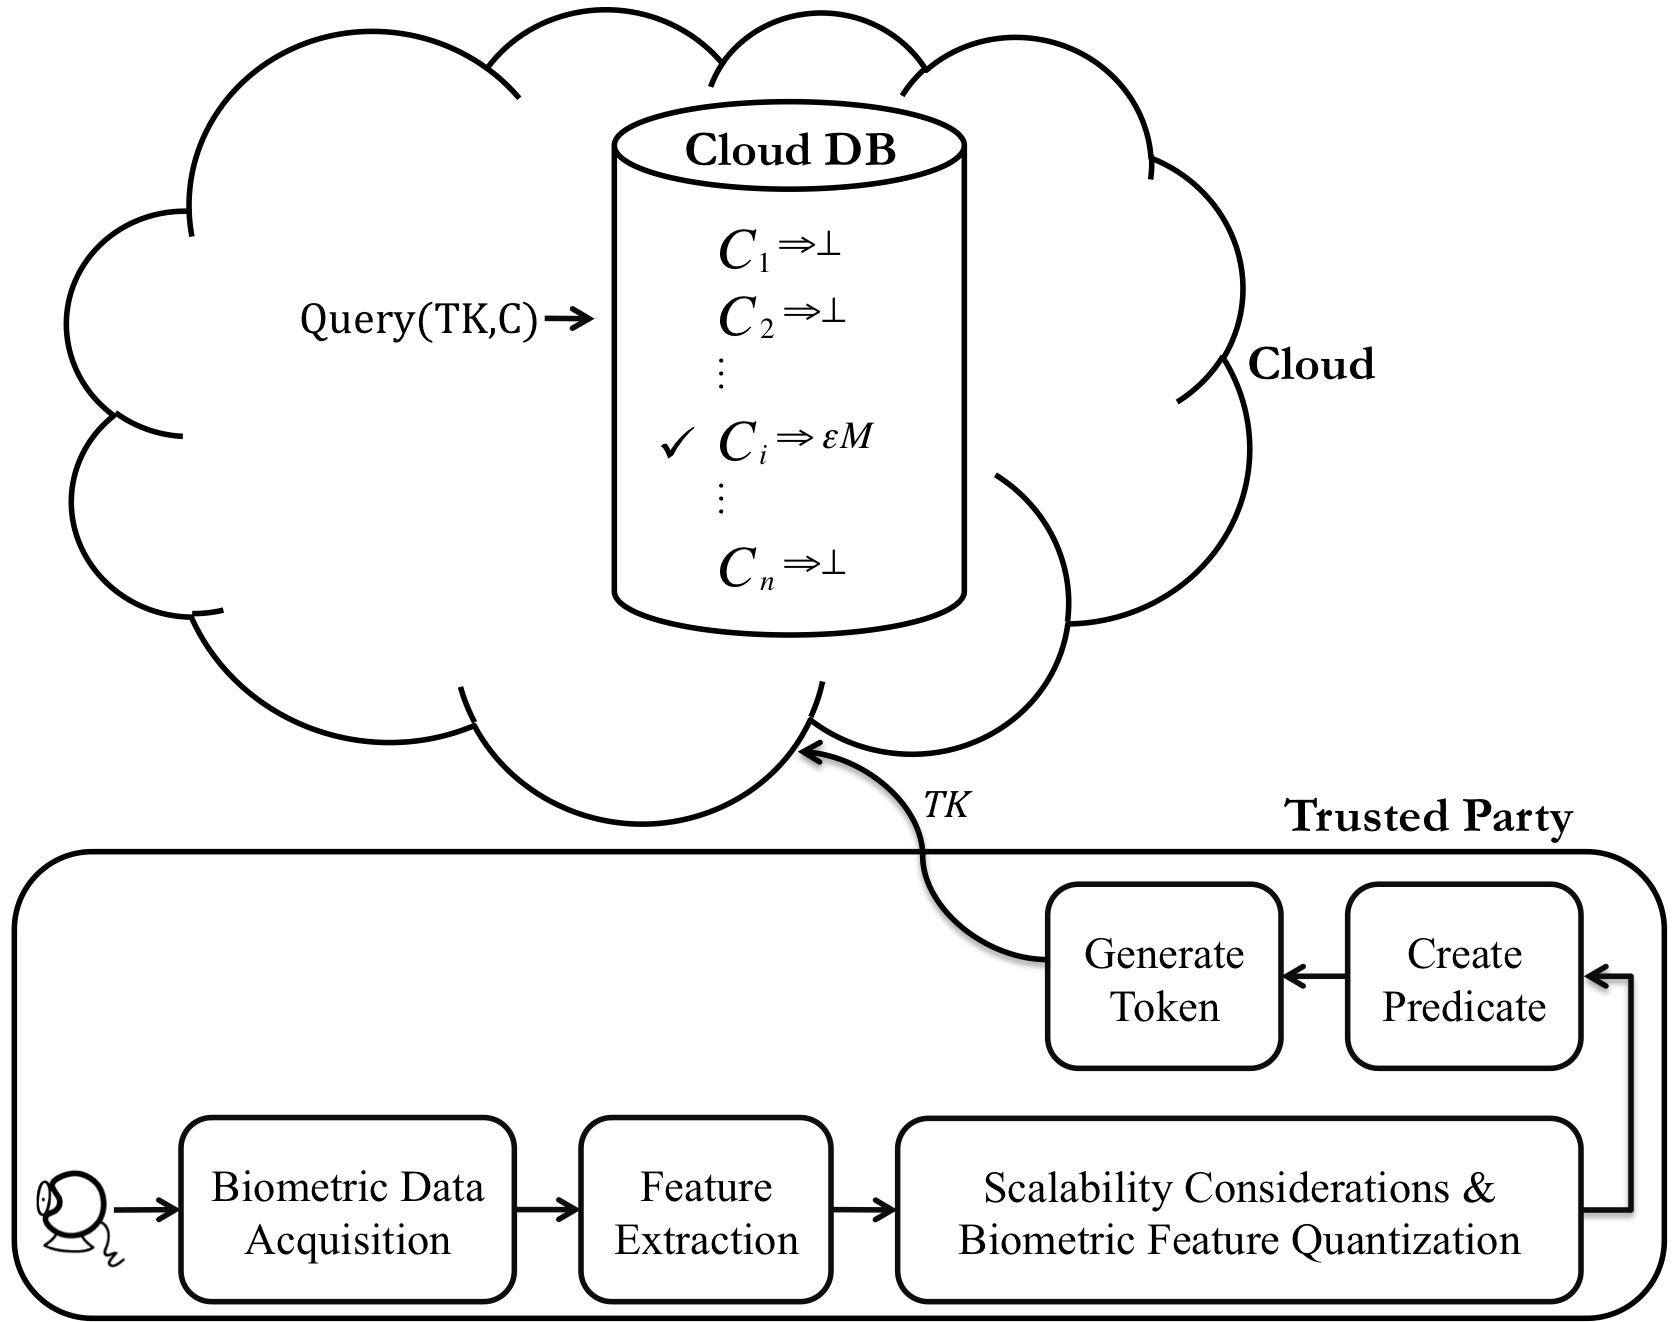
\includegraphics[width=0.6\textwidth]{./Figures/big-picture.png}
\caption{This is where the caption of the figure goes.}
\label{fig:big-picture}
\end{figure}



\section{Equations} \label{sec:equation}

Section \ref{sec:equation} is just an example to show how to insert inline and numbered equations. 

The inline equations has to be inserted between two dollar signs. Some examples are: $X^{\prime}$, or $Y^{\prime}$, or $S_{xy_{(r\times r)}}^{\prime}$. 

The numbered equations, on the other hand, need to be placed in an equation environment beginning and ending as below:
%
\begin{equation} \label{eq:1}
(U \Sigma^{-1/2})^T \, S_{xy}^{\prime} \, (V \Sigma^{-1/2}) = I \,,
\end{equation}
%
which is numbered as Eq. \ref{eq:1}.

Eq. \ref{eq:2} is an example of a multi-line equation:
\begin{equation} \begin{split} \label{eq:2}
G(x,y)=\frac{f^2}{\pi\gamma\eta} exp{\left(-\frac{x'^2+\gamma^2 y'^2}{2\sigma^2}\right)} exp{\left( j2\pi f x' + \phi \right)}     \\
x' = \;\;\; xcos\theta+ysin\theta    \\
y' = -xsin\theta+ycos\theta
\end{split} \end{equation}


\begin{table}[t]
\renewcommand{\arraystretch}{1.1}
\caption{This is where the caption of the table goes.}
\label{tab:runTime}
\centering
\footnotesize
\vspace{-0.1in}
\begin{tabular}{|l|c|}
\hline
Method				& 	Run Time (in milliseconds)\\
\hline\hline
Serial + PCA + KNN 		& 	19		\\
Serial + LDA + KNN 		& 	24		\\
Parallel + PCA + KNN 		& 	39		\\
Parallel + LDA + KNN 		& 	42		\\
PCA + CCA + KNN 		& 	19		\\
LDA + CCA + KNN 		& 	21		\\
JSRC 				& 	8406		\\
SMDL				&	7882		\\
DCA + KNN 			& 	19		\\
\hline
\end{tabular}
\vspace{-0.1in}
\end{table}




\vspace{0.2in}
\section{Section Title}\label{sec:foo}

This is an example to show how to insert sections in your chapter.



\vspace{0.2in}
\subsection{SubSection Title}\label{sec:bar}

This is an example of a sub-section.
Table \ref{tab:runTime} is just an example to show how to insert tables.



\vspace{0.2in}
\subsubsection{SubSubSection Title}

This is an example of a sub-sub-section, and another Table \ref{tab:wvu}.



\begin{table}[h]
\renewcommand{\arraystretch}{1.1}
\caption{Rank-1 recognition rates for multimodal fusion of face, ear and profile face biometrics in WVU database.}
\label{tab:wvu}
\centering
\footnotesize
\vspace{-0.1in}
\begin{tabular}{|l|c|c|c|}
\hline
\diagbox{Method}{Modality}	& Face+Ear		& Ear+Profile	& \begin{tabular}[x]{@{}c@{}}Face+Ear\\+Profile\end{tabular}	\\
\hline \hline
Serial + PCA + KNN		& $89.14 \pm 1.15$ 	& $89.46 \pm 1.13$	& $92.28 \pm 1.11$ 	\\
Serial + LDA + KNN		& $94.23 \pm 1.02$ 	& $95.14 \pm 1.20$	& $95.14 \pm 1.04$ 	\\
Parallel + PCA + KNN		& $90.71 \pm 2.05$ 	& $90.61 \pm 1.86$	& 	-		\\
Parallel + LDA + KNN		& $93.38 \pm 1.66$ 	& $93.13 \pm 1.67$	& 	-		\\
PCA + CCA/MCCA + KNN		& $94.10 \pm 0.87$ 	& $94.34 \pm 0.57$	& $97.74 \pm 0.54$ 	\\
LDA + CCA/MCCA + KNN		& $94.44 \pm 0.88$ 	& $94.89 \pm 0.54$	& $97.86 \pm 0.49$ 	\\
JSRC				& $96.20 \pm 0.52$	& $97.74 \pm 0.42$	& $98.74 \pm 0.32$	\\
SMDL				& $97.24 \pm 0.48$	& $97.97 \pm 0.42$	& $99.20 \pm 0.24$	\\
DCA/MDCA + KNN			& $98.56 \pm 0.15$ 	& $99.38 \pm 0.08$ 	& $99.85 \pm 0.03$  	\\
\hline
\end{tabular}
\end{table}

\chapter{Chapter Three Title} \label{chap:2}

Chapter three goes here ...
%\input{./Sources/chapter4}
%\input{./Sources/chapter5}
\chapter{Conclusion} \label{chap:conclusion}

Conclusion goes here ...

\newpage
\appendix
\addcontentsline{toc}{chapter}{APPENDIX} % or {APPENDICES}
\section*{APPENDIX \\ Proof of the Security of the CloudID}\label{sec-appendix}

We review the proof of the security of CloudID's searchable encryption scheme presented in \cite{haghighat2015cloudid}. Let's define a security game in which an adversary is given a number of tokens and is required to distinguish two encrypted messages.
The $i^{th}$ experiment in the game proceeds as follows:

\begin{itemize}

\item \textbf{Setup} - The challenger generates the public and secret keys and $PK$ is passed to the adversary. \\
$
  PK \leftarrow (PK_1, PK_2, \cdots, PK_t)\\
  SK \leftarrow (SK_1, SK_2, \cdots, SK_t)
$

\item \textbf{Query Phase I} - The adversary adaptively requests for the tokens of the predicates $P_1, P_2, \cdots,P_{q'} \in \Phi$, and the challenger responds with the corresponding tokens\\
$TK_j \leftarrow GenToken(SK,P_j)$.

\item \textbf{Challenge} - The adversary chooses two data-biometric pairs $(M_0,B_0)$ and $(M_1,B_1)$ subject to the following restrictions:
\begin{itemize}
 \item $P_j(B_0) = P_j(B_1)$ for all $j = 1, \cdots, q'$.
 \item If $M_0 \neq M_1$, then $P_j(B_0) = P_j(B_1) = 0$ for all $j = 1, \cdots, q'$.
\end{itemize}

In $i^{th}$ experiment, the challenger constructs the following ciphertexts:

$
  C_j \leftarrow \left\{
  \begin{array}{lll}
    Encrypt(PK_j, M_0)		&\mbox{ if  $P_j(B_0) = 1$} &\mbox{ and $j \geq i$}\\
    Encrypt(PK_j, M_1)		&\mbox{ if  $P_j(B_1) = 1$} &\mbox{ and $j < i$}\\
    Encrypt(PK_j, \bot)		&\mbox{ o/w}, &
  \end{array} \right.
$

and returns $C \leftarrow (C_1, C_2, \cdots, C_t)$.

\item \textbf{Query Phase II} - The adversary can request more tokens for predicates $P_{q'+1}, \cdots,P_q \in \Phi$ as long as they
adhere to the above restrictions.

\item \textbf{Guess} - The challenger flips a coin $\beta \in \{0,1\}$ and gives $C_* = Encrypt(PK_{B_{\beta}},M_{\beta})$ to the adversary, who returns a guess $\beta' \in \{0,1\}$ of $\beta$. The advantage of adversary in attacking the system is defined as

$
Adv = |Pr(\beta = \beta')-\frac{1}{2}|.
$

\end{itemize}

If $Exp^i$ is the probability that the adversary guesses $\beta' = 1$ in experiment $i$, in a chain of $t+1$ experiments, the adversary's advantage can be calculated by the differences in the outer experiments

$
Adv = |Exp^1 - Exp^{t+1}| \leq \sum \limits_{i=1}^t|Exp^i - Exp^{i+1}| .
$

Since the public key system is semantically secure, $|Exp^i - Exp^{i+1}|$ and consequently adversary's advantage are negligible, which make the $\Phi$-searchable system secure.


\baselineskip 0.2in
%\bibliographystyle{amsalpha}
\bibliographystyle{IEEEtran}
\bibliography{./Sources/references}

\end{document}